%%%%%%%%%%%%%%%%%%%%%%%%%%%%%%%%%%%%%%%%%%%%%%%%%%
%% Bachelor's & Master's Thesis Template        %%
%% Copyleft by Dawid Weiss & Marta Szachniuk    %%
%% Faculty of Computing and Telecommunication   %%
%% Poznan University of Technology, 2020        %%
%%%%%%%%%%%%%%%%%%%%%%%%%%%%%%%%%%%%%%%%%%%%%%%%%%


% Szkielet dla pracy licencjackiej pisanej w języku polskim.

\documentclass[polish,bachelor,a4paper,oneside]{ppfcmthesis}


\usepackage[utf8]{inputenc}
\usepackage[T1]{fontenc}
\usepackage{svg}
\usepackage{float}
\usepackage{minted}

%--------------------------------------
% Strona tytułowa
%--------------------------------------

% Autorzy pracy, jeśli jest ich więcej niż jeden
% wstaw między nimi separator \and
\author{%
   Szymon Krzysztof Gogulski \album{147403}
}
\authortitle{}                                % Do not change.

\title{Temat pracy dyplomowej}

% Your supervisor comes here.
\ppsupervisor{dr inż.~Michał Melosik} 

% Year of final submission (not graduation!)
\ppyear{2026}                                 


\begin{document}

% Front matter starts here
\frontmatter\pagestyle{empty}%
\maketitle\cleardoublepage%

%--------------------------------------
% Miejsce na kartę pracy dyplomowej
%--------------------------------------

\thispagestyle{empty}\vspace*{\fill}%
\begin{center}Tutaj będzie karta pracy dyplomowej;\\oryginał wstawiamy do wersji dla archiwum PP, w pozostałych kopiach wstawiamy ksero.\end{center}%
\vfill\cleardoublepage%

%--------------------------------------
% Spis treści
%--------------------------------------

\pagenumbering{Roman}\pagestyle{ppfcmthesis}%
\tableofcontents* 

% Spis rysunków
\listoffigures*
% Spis tabel
\listoftables*

\cleardoublepage % Zaczynamy od nieparzystej strony


%--------------------------------------
% Rozdziały
%--------------------------------------

%Najwygodniej jeśli każdy rozdział znajduje się w oddzielnym pliku
\mainmatter%

\chapter{Wstęp}

% Wstęp do pracy powinien zawierać następujące elementy:
% \begin{itemize}
%     \item krótkie uzasadnienie podjęcia tematu; 
%     \item cel pracy (patrz niżej); 
%     \item zakres (przedmiotowy, podmiotowy, czasowy) wyjaśniający, w jakim rozmiarze praca będzie realizowana; 
%     \item ewentualne hipotezy, które autor zamierza sprawdzić lub udowodnić; 
%     \item krótką charakterystykę źródeł, zwłaszcza literaturowych; 
%     \item układ pracy (patrz niżej), czyli zwięzłą charakterystykę zawartości poszczególnych rozdziałów; 
%     \item ewentualne uwagi dotyczące realizacji tematu pracy np.~trudności, które pojawiły się w trakcie 
%     realizacji poszczególnych zadań, uwagi dotyczące wykorzystywanego sprzętu, współpraca z firmami zewnętrznymi. 
% \end{itemize}

% \begin{figure}[h]
%     \centering
%     
\includegraphics[width=0.4\textwidth]{figures/images.png}
%     \caption{Schemat przedstawiający koncepcję systemu}
%     \label{fig:1}
% \end{figure}

% \noindent
% \textbf{Wstęp do pracy musi się kończyć dwoma następującymi akapitami:}
% \begin{quote}
% Celem pracy jest opracowanie / wykonanie analizy / zaprojektowanie / ...........
% \end{quote}
% oraz:
% \begin{quote}
% Struktura pracy jest następująca. W rozdziale 2 przedstawiono przegląd literatury na temat ........ 
% Rozdział 3 jest poświęcony ....... (kilka zdań). 
% Rozdział 4 zawiera ..... (kilka zdań) ............ itd. 
% Rozdział X stanowi podsumowanie pracy. 
% \end{quote}

% W przypadku prac inżynierskich zespołowych lub magisterskich 2-osobowych, po tych dwóch w/w akapitach 
% musi w pracy znaleźć się akapit, w którym będzie opisany udział w pracy poszczególnych członków zespołu. Na przykład:

% \begin{quote}
% Jan Kowalski w ramach niniejszej pracy wykonał projekt tego i tego, opracował ......
% Grzegorz Brzęczyszczykiewicz wykonał ......, itd. 
% \end{quote}

\section{Zapotrzebowanie na niezawodne źródła losowości}

\noindent Generatory liczb losowych stanowią podstawę dla algorytmów nowoczesnej 
kryptografii~\cite{2016Sreekumar-Ramesh}. Generowanie par kluczy kryptograficznych 
oraz tworzenie podpisów cyfrowych nie byłyby możliwe bez odpowiednich źródeł 
losowości. Równocześnie generatory liczb losowych nie spełniające metryk 
statystycznych oraz miar losowości będą osłabiać skuteczność algorytmów. 
Przesłanki te stanowią motywację do podjęcia badań związanych z oceną dostępnych generatorów. 

\section{Cel pracy}

\noindent Celem tej pracy magisterskiej jest implentacja oraz badanie generatorów losowości 
bazujących na oscylatorach pierścieniowych. Badane moduły będą implementowane w postaci 
układów cyfrowych realizowanych na płytach deweloperskich wyposażonych w układy FPGA. 
Na kryteria oceny generatorów będą składać się zbiór testów statystycznych związany z 
publikacją NIST SP 800-22~\cite{NIST-SP-800-22}, zbiór testów do oceny entropii 
związany z publikacją NIST SP 800-90B~\cite{NIST-SP-800-90B} oraz program do 
oceny generatorów pseudolosowych ENT~\cite{fourmilab-ENT}. 

Wraz z wynikami testów zestawione zostaną informacje o zajętość sprzętowej poszczególnych 
implementacji. Poszczególne badane moduły będą stanowić modyfikację bazowego 
modułu neoTRNG przedstawionego w repozytorium~\cite{neoTRNG}. Modyfikacje obejmą 
obszary: ilościowe (ilość zastosowanych oscylatorów), korekcji źródła 
(wpływ korektora Von-Neumana), metod post-processing'u oraz 
fizycznego rozmieszczenia w FPGA. 

Osobna faza odporności i monitorowania przetestuje zastosowanie modułów testowych 
(Health Test) oraz wpływ warunków środowiskowych na jakość badanego źródła entropii.

Dodatkowy etap implementacyjny porówna zastosowanie neoTRNG jako generator entropii dla 
komputera jednopłytkowego RPI oraz zestawi to rozwiązanie z komercyjnym modułem Quantis.

% \begin{enumerate}
%     \item Zestaw wszystkie założenia pracy
%     \item Przedstaw badane obszary projektowanego źródła (zajętość, testy, analiza rozmieszczenia ...)
% \end{enumerate}

\section{Charakterystyka literatury}

Poszczególne badania zostana przeprowadzone stosując rekomendacje branżowe odnośnie 
projektowania źródeł entropii oraz publikacje akademickie związane z tematem. 

\section{Układ pracy}

Struktura pracy podzielona jest osiem rozdziałów oraz osobną sekcję z załącznikami.
Rozdział pierwszy wyjaśnia motywację podjęcia badań w obszarze generatorów entropii 
oraz zestawia założenia i cele pracy dyplomowej. Rodział drugi skupia się na wyjaśnieniu 
podstaw teorertycznych, w ramach których omówione zostaną podstawowe definicje 
związane z tematyką pracy, przedstawiona zostanie architektura badanego źródła entropii, 
a także objaśnione zostaną szczegóły metod korekcji źródła, kompresji entropii oraz 
metody badania źródła entropii (zestawy testów oraz moduły testowe). Rodział trzeci 
będzie stanowić rozpoczęcie prac badawczych: zbadany zostanie wpływ stosowania 
korekcji źródła oraz kompresji entropii na poziom entropii oraz zajętość układu. 


\chapter{Teoretyczne aspekty projektowania sprzętowych generatorów liczb losowych}

% Rozdział teoretyczny --- przegląd literatury naświetlający stan wiedzy na dany temat. 

% Przegląd literatury naświetlający stan wiedzy na dany temat obejmuje rozdziały pisane na podstawie
% literatury, której wykaz zamieszczany jest w części pracy pt.~\emph{Literatura} (lub inaczej \emph{Bibliografia},
% \emph{Piśmiennictwo}). W tekście pracy muszą wystąpić odwołania do wszystkich pozycji zamieszczonych w
% wykazie literatury. \textbf{Nie należy odnośników do literatury umieszczać w stopce strony.} Student jest
% bezwzględnie zobowiązany do wskazywania źródeł pochodzenia informacji przedstawianych w pracy,
% dotyczy to również rysunków, tabel, fragmentów kodu źródłowego programów itd. Należy także podać
% adresy stron internetowych w przypadku źródeł pochodzących z Internetu.

\noindent Niniejszy rozdział przedstawia teoretyczne podstawy projektoawnia 
sprzętowych generatorów liczb losowych. Omówiona zostanie klasyfikacja architektur generatorów 
oraz fizyczne zjawiska wykorzystywane do pozyskiwania entropii w układach programowalnych 
FPGA. Ponadto wytłumaczne zostaną metody obróbki sygnałów losowych oraz 
standardy statystyczne stosowane do walidacji jakości generowanych danych.

\section{Źródła losowości}



\subsection{TRBG}

\begin{figure}[H]
    \centering
    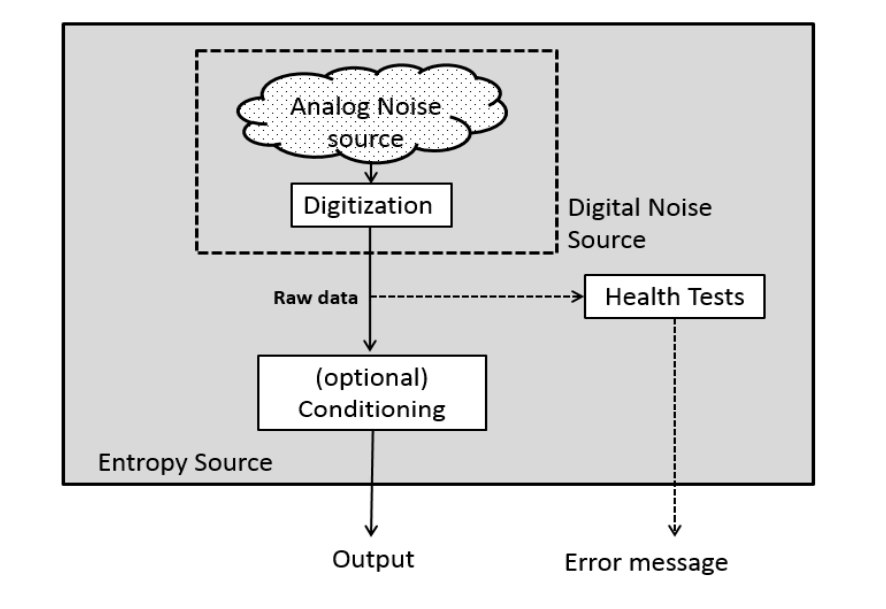
\includegraphics[width=0.75\textwidth]{figures/ch2/nist_source_schematic.png}
    \caption{Model źródła entropii. \cite{NIST-SP-800-90B}}
    \label{fig:ch2_model_zrodla_entropii_nist}
\end{figure}

\subsection{PRBG}

\subsection{QRBG}

\subsection{Zasada działania Quantis USB 4M}

\section{RO jako źródła losowości w FPGA}

\begin{figure}[H]
    \centering
    \includesvg[width=\textwidth]{figures/ch2/schematic.svg}
    \caption{Przykład prostego oscylatora pierścieniowego.}
    \label{fig:ch2_oscylator_3xNOT}
\end{figure}

\section{Ekstraktory losowości}

\subsection{Ekstraktor von Neumanna}

\subsection{Wielomian CRC}

\subsection{Ekstraktor Toeplitz'a}

\subsection{Szyfr strumieniowy AES-CTR}

\section{Metody oceny losowości}

\subsection{ENT - Fourmilab Random Sequence Tester}

\subsection{NIST SP 800-22 - A Statistical Test Suite for Random and Pseudorandom Number Generators for Cryptographic Applications}

\subsection{NIST SP 800-90B - Entropy Assessment Test Suite}

 
% Rozdziały dokumentujące pracę własną studenta: opisujące ideę, sposób lub metodę 
% rozwiązania postawionego problemu oraz rozdziały opisujące techniczną stronę rozwiązania 
% --- dokumentacja techniczna, przeprowadzone testy, badania i uzyskane wyniki. 

% Praca musi zawierać elementy pracy własnej autora adekwatne do jego wiedzy praktycznej uzyskanej w
% okresie studiów. Za pracę własną autora można uznać np.: stworzenie aplikacji informatycznej lub jej
% fragmentu, zaproponowanie algorytmu rozwiązania problemu szczegółowego, przedstawienie projektu 
% np.~systemu informatycznego lub sieci komputerowej, analizę i ocenę nowych technologii lub rozwiązań
% informatycznych wykorzystywanych w przedsiębiorstwach, itp. 

% Autor powinien zadbać o właściwą dokumentację pracy własnej obejmującą specyfikację założeń i 
% sposób realizacji poszczególnych zadań
% wraz z ich oceną i opisem napotkanych problemów. W przypadku prac o charakterze 
% projektowo-implementacyjnym, ta część pracy jest zastępowana dokumentacją techniczną i użytkową systemu. 

% W pracy \textbf{nie należy zamieszczać całego kodu źródłowego} opracowanych programów. Kod źródłowy napisanych
% programów, wszelkie oprogramowanie wytworzone i wykorzystane w pracy, wyniki przeprowadzonych
% eksperymentów powinny być umieszczone np. na płycie CD, stanowiącej dodatek do pracy.

% \section*{Styl tekstu}

% Należy\footnote{Uwagi o stylu pochodzą częściowo ze stron prof. Macieja Drozdowskiego~\cite{Drozdowski2006}.} 
% stosować formę bezosobową, tj.~\emph{w pracy rozważono ......, 
% w ramach pracy zaprojektowano ....}, a nie: \emph{w pracy rozważyłem, w ramach pracy zaprojektowałem}. 
% Odwołania do wcześniejszych fragmentów tekstu powinny mieć następującą postać: ,,Jak wspomniano wcześniej, ....'', 
% ,,Jak wykazano powyżej ....''. Należy unikać długich zdań. 

% Niedopuszczalne są zwroty używane w języku potocznym. W pracy należy używać terminologii informatycznej, która ma 
% sprecyzowaną treść i znaczenie. 

% Niedopuszczalne jest pisanie pracy metodą \emph{cut\&paste}, bo jest to plagiat i dowód intelektualnej indolencji autora.
% Dane zagadnienie należy opisać własnymi słowami. Zawsze trzeba powołać się na zewnętrzne źródła. 

% ////////////////////////////////////////////////////////////////////////////////////////
% 1. Interfejsy i testy bazowe
% • Implementacja bazowego projektu neoTRNG na układzie FPGA.
% • Uruchomienie komunikacji:
% • interfejs UART
% • moduł pMOD SD Card (szybki zapis surowych bitów bezpośrednio do
% sektorów karty, bez systemu plików, przez interfejs SPI).
% • Przygotowanie środowiska analitycznego na komputerze PC: instalacja i
% konfiguracja pakietu ent, zestawu testów statystycznych NIST SP 800-22 oraz
% narzędzia do estymacji min-entropii NIST SP 800-90B. (bez/z de-biassing, bez/z
% CRC (z obecnym de-biasing))

\chapter{Testy bazowe}

\noindent W niniejszym rozdziale przeanalizowano wpływ zastosowania korekcji źródła oraz 
przetwarzania końcowego na poziom generowanej entropii w domyślnej implementacji 
neoTRNG. Rozważane elementy architektury zostały przedstawione na rysunku 
\ref{fig:architektura_neotrng} jako moduły „de-biasing” oraz „sampling”. W 
implementacji bazowej zastosowano korektor von Neumanna oraz mechanizm kompresji 
entropii oparty na CRC. W ramach przeprowadzonych testów porównano cztery 
warianty konfiguracji generatora:

\begin{enumerate}
    \item moduł z korektorem von Neumanna oraz CRC (domyślny),
    \item moduł z korektorem von Neumanna bez CRC,
    \item moduł bez korektora z aktywnym CRC,
    \item moduł bez korektora i bez CRC.
\end{enumerate}

Zbadane zostały kolejno moduły z:

\begin{enumerate}
    \item trzema pętlami oscylatorów po 5, 7 oraz 9 inwerterów,
    \item trzema pętlami oscylatorów po 3, 5 oraz 7 inwerterów,
    \item dwiema pętlami oscylatorów po 3 i 5 inwerterów.
\end{enumerate}

\section{Modyfikacja}

\noindent Testy przeprowadzono na zmodyfikowanym module neoTRNG. Moduł rozszerzono o dwa parametry generyczne
 \textit{ENABLE\_VON\_NEUMANN} oraz \textit{ENABLE\_CRC} w celu łatwej konfiguracji. Zmodyfikowany plik źródłowy znajduje się w załączniku
  A neoTRNG\_mod\_1.vhd.

Każdy z przypadków testowych uruchomiono na sprzęcie, a uzyskane wyniki zapisano w odpowiednich plikach.


\section{ENT}

\begin{table}[H]
\centering
\caption{ENT: Entropy bits per byte.}
\label{tab:ch3_ent}
\begin{tabular}{|l|c|c|c|c|}
\hline
\textbf{Konfiguracja} & \textbf{3RO 5-7-9} & \textbf{3RO 3-5-7} & \textbf{2RO 3-5} \\ \hline
\textbf{true/true}      & 7.999998 & 7.999998 & 7.999997 \\ \hline
\textbf{true/false}     & 7.928600 & 7.856006 & 7.368478 \\ \hline
\textbf{false/true}     & 7.999988 & 7.999995 & 7.999742 \\ \hline
\textbf{false/false}    & 7.404643 & 7.921076 & 7.617650 \\ \hline
\end{tabular}
\end{table}

\section{NIST SP 800-22}

\begin{flushleft}
\small \textbf{Note:} The minimum pass rate for each statistical test with the exception of the
random excursion (variant) test is approximately = 96 for a
sample size = 100 binary sequences\cite{NIST-SP-800-22}. \\
\small \textbf{Note:} The minimum pass rate for each statistical test with the exception of the
random excursion (variant) test is approximately = 96 for a
sample size = 100 binary sequences\cite{NIST-SP-800-22}. \\
\small \textbf{Legend:} \textbf{sp} - subtests passed (zaliczone podtesty). \\
\small \textbf{Legend:} \textbf{*} - test niezaliczony. \\
\small \textbf{Legend:} \textbf{\textit{ENABLE\_VON\_NEUMANN}/ \textit{ENABLE\_CRC}} - wybrana konfiguracja.
\end{flushleft}

\begin{table}[H]
\centering
\caption{3 RO : 5 - 7 - 9}
\label{tab:nist_22_3RO_21I}
\begin{tabular}{|l|c|l|c|l|c|l|c|l|}
\hline
\textbf{Statistical Test} & \multicolumn{2}{c|}{\textbf{true/true}} & \multicolumn{2}{c|}{\textbf{true/false}} & \multicolumn{2}{c|}{\textbf{false/true}} & \multicolumn{2}{c|}{\textbf{false/false}} \\ \hline
Frequency               &  98/100 &     & 100/100 &     &  97/100 &     & 100/100 &     \\ \hline
BlockFrequency          &  99/100 &     & 100/100 &     &  98/100 &     & 100/100 &     \\ \hline
CumulativeSums          &  98/100 &     & 100/100 &     &  97/100 &     &  99/100 &     \\ \hline
CumulativeSums          &  98/100 &     & 100/100 &     &  97/100 &     & 100/100 &     \\ \hline
Runs                    & 100/100 &     &   0/100 & *   &  97/100 &     &   0/100 & *   \\ \hline
LongestRun              & 100/100 &     &   0/100 & *   &  99/100 &     &   0/100 & *   \\ \hline
Rank                    &  99/100 &     &  99/100 &     &  99/100 &     &  99/100 &     \\ \hline
FFT                     & 100/100 &     &   2/100 & *   &  98/100 &     &   0/100 & *   \\ \hline
NonOverlappingTemplate  & 147/148 & sp  &   8/148 & sp  & 148/148 & sp  &   0/148 & sp  \\ \hline
OverlappingTemplate     & 100/100 &     &   0/100 & *   &  99/100 &     &   0/100 & *   \\ \hline
Universal               &  97/100 &     &   0/100 & *   & 100/100 &     &   0/100 & *   \\ \hline
ApproximateEntropy      & 100/100 &     &   0/100 & *   & 100/100 &     &   0/100 & *   \\ \hline
RandomExcursions        &     7/8 & sp  &     1/8 & sp  &     8/8 & sp  &     2/8 & sp  \\ \hline
RandomExcursionsVariant &   18/18 & sp  &   18/18 & sp  &   18/18 & sp  &   18/18 & sp  \\ \hline
Serial                  &  99/100 &     &   0/100 & *   &  99/100 &     &   0/100 & *   \\ \hline
Serial                  &  98/100 &     &  95/100 & *   &  99/100 &     &   0/100 & *   \\ \hline
LinearComplexity        &  99/100 &     &  99/100 &     & 100/100 &     & 100/100 &     \\ \hline
\end{tabular}
\end{table}

\begin{table}[H]
\centering
\caption{3 RO : 3 - 5 - 7}
\label{tab:nist_22_3RO_15I}
\begin{tabular}{|l|c|l|c|l|c|l|c|l|}
\hline
\textbf{Statistical Test} & \multicolumn{2}{c|}{\textbf{true/true}} & \multicolumn{2}{c|}{\textbf{true/false}} & \multicolumn{2}{c|}{\textbf{false/true}} & \multicolumn{2}{c|}{\textbf{false/false}} \\ \hline
Frequency               &  98/100 &     &  96/100 &     &  98/100 &     &  94/100 & *   \\ \hline
BlockFrequency          & 100/100 &     &   0/100 & *   &  97/100 &     &   0/100 & *   \\ \hline
CumulativeSums          &  98/100 &     &  93/100 & *   &  99/100 &     &  93/100 & *   \\ \hline
CumulativeSums          &  99/100 &     &  93/100 & *   &  98/100 &     &  95/100 & *   \\ \hline
Runs                    & 100/100 &     &   0/100 & *   &  98/100 &     &  84/100 & *   \\ \hline
LongestRun              &  99/100 &     &   0/100 & *   &  99/100 &     &  77/100 & *   \\ \hline
Rank                    &  99/100 &     &  98/100 &     & 100/100 &     &  97/100 &     \\ \hline
FFT                     &  98/100 &     &   0/100 & *   &  99/100 &     &   7/100 & *   \\ \hline
NonOverlappingTemplate  & 147/148 & sp  &   0/148 & sp  & 148/148 & sp  &  11/148 & sp  \\ \hline
OverlappingTemplate     & 100/100 &     &   0/100 & *   &  99/100 &     &   1/100 & *   \\ \hline
Universal               &  98/100 &     &   0/100 & *   &  96/100 &     &   0/100 & *   \\ \hline
ApproximateEntropy      & 100/100 &     &   0/100 & *   &  99/100 &     &   0/100 & *   \\ \hline
RandomExcursions        &     8/8 & sp  &     0/8 & sp  &     8/8 & sp  &     4/8 & sp  \\ \hline
RandomExcursionsVariant &   18/18 & sp  &   18/18 & sp  &   18/18 & sp  &   18/18 & sp  \\ \hline
Serial                  &  99/100 &     &   0/100 & *   &  98/100 &     &   0/100 & *   \\ \hline
Serial                  &  99/100 &     &  20/100 & *   &  99/100 &     &  94/100 & *   \\ \hline
LinearComplexity        &  97/100 &     &  98/100 &     & 100/100 &     &  99/100 &     \\ \hline
\end{tabular}
\end{table}

\begin{table}[H]
\centering
\caption{2 RO : 3 - 5}
\label{tab:nist_22_2RO_8I}
\begin{tabular}{|l|c|l|c|l|c|l|c|l|}
\hline
\textbf{Statistical Test} & \multicolumn{2}{c|}{\textbf{true/true}} & \multicolumn{2}{c|}{\textbf{true/false}} & \multicolumn{2}{c|}{\textbf{false/true}} & \multicolumn{2}{c|}{\textbf{false/false}} \\ \hline
Frequency               & 100/100 &     & 100/100 &     &  98/100 &     &  14/100 & *   \\ \hline
BlockFrequency          & 100/100 &     & 100/100 &     &  98/100 &     &   0/100 & *   \\ \hline
CumulativeSums          & 100/100 &     & 100/100 &     &  98/100 &     &  14/100 & *   \\ \hline
CumulativeSums          & 100/100 &     & 100/100 &     &  98/100 &     &  15/100 & *   \\ \hline
Runs                    & 100/100 &     &   0/100 & *   &  99/100 &     &   0/100 & *   \\ \hline
LongestRun              &  98/100 &     &   0/100 & *   &  99/100 &     &   0/100 & *   \\ \hline
Rank                    &  99/100 &     &  99/100 &     &  99/100 &     &  99/100 &     \\ \hline
FFT                     & 100/100 &     &   0/100 & *   &  98/100 &     &   0/100 & *   \\ \hline
NonOverlappingTemplate  & 148/148 & sp  &   8/148 & sp  & 148/148 & sp  &   4/148 & sp  \\ \hline
OverlappingTemplate     &  99/100 &     &   0/100 & *   & 100/100 &     &   0/100 & *   \\ \hline
Universal               &  98/100 &     &   0/100 & *   & 100/100 &     &   0/100 & *   \\ \hline
ApproximateEntropy      &  98/100 &     &   0/100 & *   &  97/100 &     &   0/100 & *   \\ \hline
RandomExcursions        &     8/8 & sp  &     0/8 & sp  &     8/8 & sp  &     0/8 & sp  \\ \hline
RandomExcursionsVariant &   18/18 & sp  &   18/18 & sp  &   18/18 & sp  &   18/18 & sp  \\ \hline
Serial                  &  99/100 &     &   0/100 & *   &  98/100 &     &   0/100 & *   \\ \hline
Serial                  & 100/100 &     &   0/100 & *   &  99/100 &     &   0/100 & *   \\ \hline
LinearComplexity        &  98/100 &     & 100/100 &     & 100/100 &     & 100/100 &     \\ \hline
\end{tabular}
\end{table}



\section{NIST SP 800-90B}



\begin{table}[H]
\centering
\caption{NIST SP 800-90: Non-IID entropy assessment}
\label{tab:ch3_NIST_SP_800_90}
\begin{tabular}{|l|c|c|c|c|}
\hline
\textbf{Konfiguracja} & \textbf{3RO 5-7-9} & \textbf{3RO 3-5-7} & \textbf{2RO 3-5} \\ \hline

\textbf{true/true} &  
\shortstack{$H_{orig}=7.918$ \\ $H_{bit}=0.941$} & 
\shortstack{$H_{orig}=$ \\ $H_{bit}=$} & 
\shortstack{$H_{orig}=$ \\ $H_{bit}=$} \\ \hline

\textbf{true/false} &
\shortstack{$H_{orig}=6.653213$ \\ $H_{bit}=0.754510$} &
\shortstack{$H_{orig}=$ \\ $H_{bit}=$} &
\shortstack{$H_{orig}=$ \\ $H_{bit}=$} \\ \hline

\textbf{false/true} &
\shortstack{$H_{orig}=7.915044$ \\ $H_{bit}=0.941182$} &
\shortstack{$H_{orig}=$ \\ $H_{bit}=$} &
\shortstack{$H_{orig}=$ \\ $H_{bit}=$} \\ \hline

\textbf{false/false} &
\shortstack{$H_{orig}=$ \\ $H_{bit}=$} &
\shortstack{$H_{orig}=$ \\ $H_{bit}=$} &
\shortstack{$H_{orig}=$ \\ $H_{bit}=$} \\ \hline
\end{tabular}
\end{table}















% 2. Analiza Rozmieszczenia (Placement)
% • Badanie wpływu fizycznej lokalizacji oscylatorów na krzemie na stopień ich
% niezależności i czystą entropię.
% • Przygotowanie konfiguracji z różną liczbą oscylatorów pierścieniowych (RO): 8, 16,
% 64 oraz 128 jednostek. (dobrać wartości tak aby uchwycić jakąś różnicę)
% • Realizacja dwóch skrajnych wariantów rozmieszczenia: Localized (bloki RO
% upakowane ciasno w jednym obszarze CLB) oraz Distributed (rozmieszczenie
% rozproszone po całej strukturze FPGA przy użyciu ograniczeń
% projektowych/constraints).
% • Pomiary bazowe: zużycie zasobów logicznych (liczba tablic LUT), średni cykl
% oscylacji poszczególnych RO, Min-entropia ($H_{min}$) oraz entropia Shannona
% (pakiet ent).
% • TABELA 1: Wpływ fizycznego rozmieszczenia na źródło entropii.
% • Zawartość: Liczba RO | Typ rozmieszczenia (Loc/Dist) | Liczba LUT | Wynik
% $H_{min}$ | Entropia wg ent.
% • Cel: Wykazanie występowania korelacji przestrzennej i jej wpływu na jakość
% generowanego szumu.

\chapter{Analiza rozmieszczenia}
% 3. Faza Algorytmiczna i Optymalizacja Ekstrakcji
% • Wybór najbardziej efektywnej metody post-processingu (tzw. wybielania) przy stałej
% liczbie źródeł (np. 64 RO).
% • Modyfikacja jednostki próbkowania (Sampling Unit) i implementacja wymiennych
% modułów:
% • XOR (rozwiązanie o najniższym koszcie sprzętowym).
% • CRC (standardowa metoda zaimplementowana w neoTRNG).
% • Toeplitz Extractor
% • AES-256 lub sha256
% • Pomiary wydajnościowe: przepustowość wyjściowa (Bitrate w Mbps), dodatkowe
% zużycie zasobów przez sam ekstraktor, pełna weryfikacja statystyczna NIST 800-22.
% • TABELA 2: Efektywność post-processingu i współczynnik $\eta$.
% • Zawartość: Typ ekstraktora | Dodatkowe LUT | Przepustowość [Mbps] |
% Wynik NIST 800-22 (Pass/Fail) | Współczynnik $\eta$ (Efektywność).

\chapter{Faza algorytmiczna i optymalizacja ekstrakcji}

% 4. Faza Odporności i Monitorowanie Online (Health Tests)
% • wpięcie modułów testowych RCT (Repetition Count Test) oraz APT (Adaptive
% Proportion Test) w torze sygnałowym przed ekstraktorem.
% • Badania środowiskowe: monitorowanie pracy układu podczas nagrzewania
% (suszarka) oraz chłodzenia (zamrażacz).
% • TABELA 4: Reakcja mechanizmów Health Test na czynniki zewnętrzne.
% • Zawartość: Temperatura pracy [°C] | Surowa wartość $H_{min}$ | Stan flagi
% Alarm (Tak/Nie) | Opóźnienie reakcji | Skuteczność ekstraktora w warunkach
% stresu.
\chapter{Faza odporności i monitorowanie online}
% • jako osobny TRBG
% • porównaieni z Quantis

\chapter{neoTRNG na FPGA dla RPI}
\input{chapters/08-zakonczenie.tex}

%--------------------------------------
% Literatura
%--------------------------------------

{\raggedright\sloppy\small
\bibliographystyle{plain}
\bibliography{bibliografia}
}
%--------------------------------------
% Dodatki
%--------------------------------------

\cleardoublepage\appendix%
\newpage
\chapter{Floorplanning}

\noindent Analiza rozmieszczenia została wykonana za pomocą narzędzia do 
palnowania rozmieszczenia logiki wewnątrz układu scalonego 
(ang. \textit{floorplanning}). 


W narzędziu Vivado

Podstawą dla przeprowadzenia analizy jest badanie generatora losowości neoTRNG. 
Generatora został zbadany przy użyciu testów losowości: NIST SP 800-22, NIST SP 800-90B 
oraz testu ENT. 

Zbadałem różne aspekty generatora i na podstawie testów próbuję określić 
ich wpływ na jakość genrowanej losowości. Badane aspekty obejmują:

- ilość wykorzystanych oscylatorów pierścieniowych (RO) oraz inwerterów (I) w oscylatorach. 
(Jak skalowanie tych parametrów wpływa na losowość?)

- zastosowanie bądź brak zastosowania korektora von Neumanna i mieszania wielomianem CRC.
(Jak obecność tych metod post-processingu wpływa na losowość?)

- rozmieszczenie RO w układzie FPGA (rozproszone - RO zdala od siebie bądź 
zlokalizowane - RO blisko siebie).
(Jak położenie RO w układzie wpłynie na losowość?)

- zastosowanie innych metod post-processingu: AES-CTR lub ekstraktora Toeplitza.
(Jak te metody post-processing wpłyną na losowość?)

do każdego z pytań muszę wyciągnąć wniosek poparty wynikami w tabelach. Muszę 
stwierdzić czy dany aspekt ma wpływ na losowość, nie ma wpływu na losowość bądź 
wynik nie jest jednoznaczny. 


%--------------------------------------
% Informacja o prawach autorskich
%--------------------------------------



\ppcolophon

\end{document}
